% Created 2019-12-19 Thu 11:54
% Intended LaTeX compiler: pdflatex
\documentclass[11pt]{article}
\usepackage[utf8]{inputenc}
\usepackage[T1]{fontenc}
\usepackage{graphicx}
\usepackage{grffile}
\usepackage{longtable}
\usepackage{wrapfig}
\usepackage{rotating}
\usepackage[normalem]{ulem}
\usepackage{amsmath}
\usepackage{textcomp}
\usepackage{amssymb}
\usepackage{capt-of}
\usepackage{hyperref}
\usepackage[a4paper,total={6.5in, 9.5in}]{geometry}
\usepackage{minted}
\setminted{fontsize=\footnotesize}
\usepackage[font={small,sf},labelfont=bf,format=hang,format=plain,margin=0pt,width=0.8\textwidth,]{caption}
\author{Jakub Zárybnický (xzaryb00), Jan Hammer (xhamme00)}
\date{19. 12. 2019}
\title{Implementace metod získávání znalostí\\\medskip
\large Řešení}
\begin{document}

\maketitle

\section{Zadání}
\label{sec:org7d3e019}
Kohonenova mapa (self-organizing map, SOM) je typ neuronové sítě trénovaný
pomocí učení bez učitele (unsupervised learning). Používá se pro snížení
dimenzionality dat, často pro projekci do 2D/3D prostoru za účelem
vizualizace. Také se používá pro klasifikační úkoly, kdy výsledkem učení jsou
shluky. Podobnými metodami jsou k-means clustering nebo support vector machines,
které mohou dostávat lepší výsledky v klasifikačních úkolech, ale zato nemají
tak čitelné vizualizační výstupy.

Cílem našeho projektu bylo implementovat Kohonenovu mapu i vizualizace nad ní a
demonstrovat funkčnost nad několika sadami dat.

\section{Přístup}
\label{sec:orgae4c599}
Mapu jsme implementovali v jazyce Python pomocí knihovny pro práci s maticemi
Numpy. Pro vizualizaci jsme použili další knihovnu - ne maplotlib, jak bylo
původně v plánu, ale hlavně kvůli animacím jsme použili graphics-py. Poslední
externí knihovna, použitá čistě z pohodlnosti, je Click, knihovna pro tvorbu
rozhraní příkazové řádky.

Vytvořili jsme knihovnu a aplikaci skládající se ze dvou modulů \texttt{som.map} a
\texttt{som.graphics} a ze spustitelné aplikace \texttt{som.py}. Aplikace obsahuje tři oddělené
příkazy - \texttt{generate} pro generování náhodných dat (volitelně ve shlucích), \texttt{train}
pro natrénovaní mapy s řadou nastavitelných parametrů a \texttt{visalize} pro zobrazení
již natrénovaného modelu.

Dále jsme vytvořili dva skripty \texttt{mnist.py} a \texttt{iris.py}, které demonstrují použití
API vytvořené knihovny.

\subsection{Algoritmus}
\label{sec:org812a1ea}
Jeden krok učení Kohonenovy mapy má dva podkroky:
\begin{itemize}
\item najít uzel, jehož váhové parametry jsou nejbližší aktuálně trénovanému vzorku,
tzv. BMU (Best Matching Unit)
\item a posunout takto nalezený uzel a jeho sousedy blíže k trénovanému vzorku s
vahou odpovídající obrácené vzdálenosti souseda od BMU (používáme tzv. \emph{Manhattan distance}).
\end{itemize}

\newpage

\section{Výsledky}
\label{sec:org697099a}

\subsection{Random}
\label{sec:org7730a1c}
\begin{minted}[]{shell}
./som.py generate 20 > random.csv
./som.py train --animate --animate-interval 5 \
  --size 10x10 --rate 0.2 --epochs 15 -m random.npz \
  random.csv
./som.py visualize random.npz
\end{minted}

První příkaz vygeneruje 20 náhodných vzorků o délce 2, druhý nad nimi natrénuje
síť o velikosti 10x10 a zároveň při tréninku zobrazuje animaci, jak se síť mění
při učení. Natrénovanou síť uloží do souboru, odkud ji pak načte poslední
příkaz, který vizualizuje už netrénovanou síť.

\begin{center}
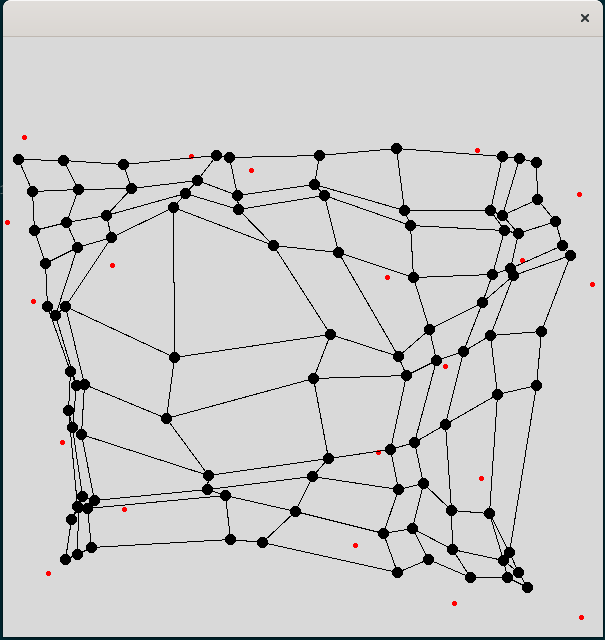
\includegraphics[width=.7\linewidth]{img/Screenshot from 2019-12-19 11-27-05.png}
\end{center}

\subsection{Clusters}
\label{sec:org70edf6b}
\begin{minted}[]{shell}
./som.py generate --clusters 3 300 > clusters.csv
./som.py train --animate --animate-interval 1 \
  --size 10x10 --rate 0.2 --epochs 5 -m clusters.npz \
  clusters.csv
\end{minted}

Sada příkazů generuje sadu 300 vzorků o délce 2 seskupenou do tří shluků, nad
nimi natrénuje síť a během tréninku vizualizuje, jak se síť postupně učí.

\begin{center}
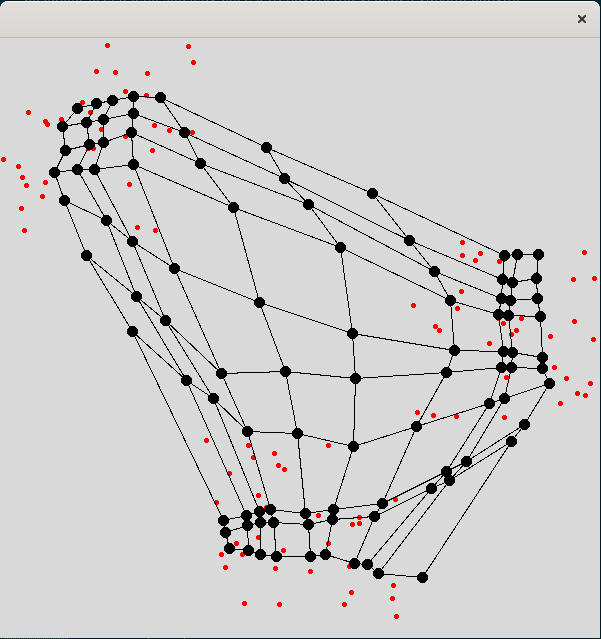
\includegraphics[width=.7\linewidth]{img/Screenshot from 2019-12-19 11-28-01.png}
\end{center}

\subsection{MNIST}
\label{sec:org3d534b8}
\begin{minted}[]{shell}
./mnist.py -S 20x20 --skip-rows 1 train.csv
\end{minted}

Program rozdělí vstupní data na testovací a trénovací množinu a pak paralelně
trénuje Kohonenovu mapu a klasifikátor na ní založený - každý uzel má ještě
váhový vektor s one-hot zakódovaným výsledkem klasifikace, který se trénuje
stejně jako mapa samotná, s propagací do sousedních uzlů.

Na závěr se program pokusí se klasifikovat data testovací množiny. Nejvyšší
procento správně klasifikovaných vzorků, co jsem viděl, bylo 76.52\% - zamícháním
tréninkových dat před začátkem učení jsou ale výsledky nedeterministické,
pravidelně dosahujeme výsledků kolem 68\% a další úpravou parametrů nebo třeba
zvětšením by bylo možné dosáhnout ještě lepších výsledků.

\begin{center}
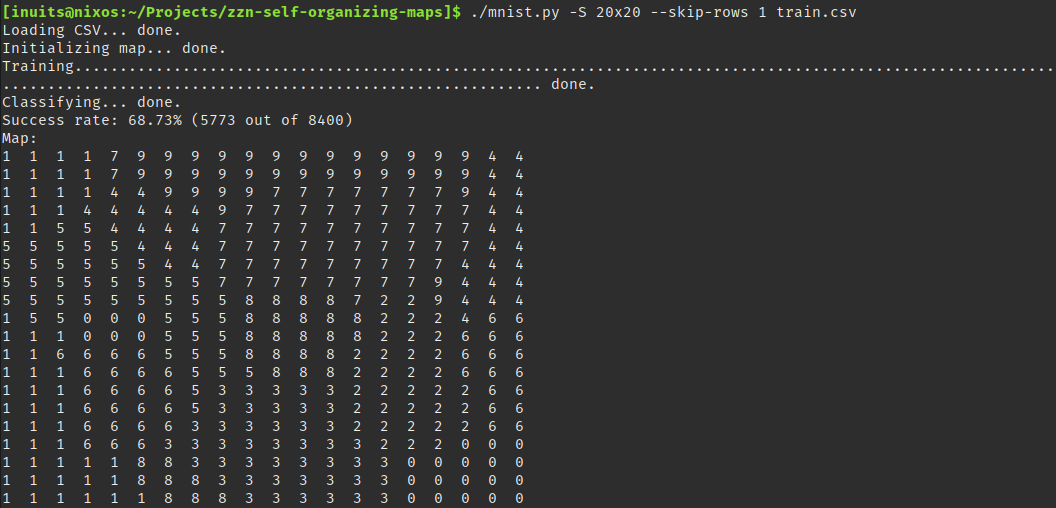
\includegraphics[width=.7\linewidth]{img/Screenshot from 2019-12-19 11-28-55.png}
\end{center}

\subsection{Iris}
\label{sec:org89c915a}
\begin{minted}[]{shell}
./iris.py -epochs 50 --size 10x10 iris-preprocessed.csv
\end{minted}

Program pracuje stejně jako \texttt{./mnist.py}, jen s lehce upraveným zpracováním
označení vzorků (labels). Při učení zobrazuje rozložení mapy v 2D prostoru -
první okno rozložení na základě lístků kališních (první dva rozměry dat), druhé
na základě listů korunních (druhé dva rozměry).

Zde s uvedenými parametry učení dosahujeme úspěšnost ověření nad testovacími
daty přes 90\% - nejlepší výsledek, co jsem viděl byl 100\%.

\begin{center}
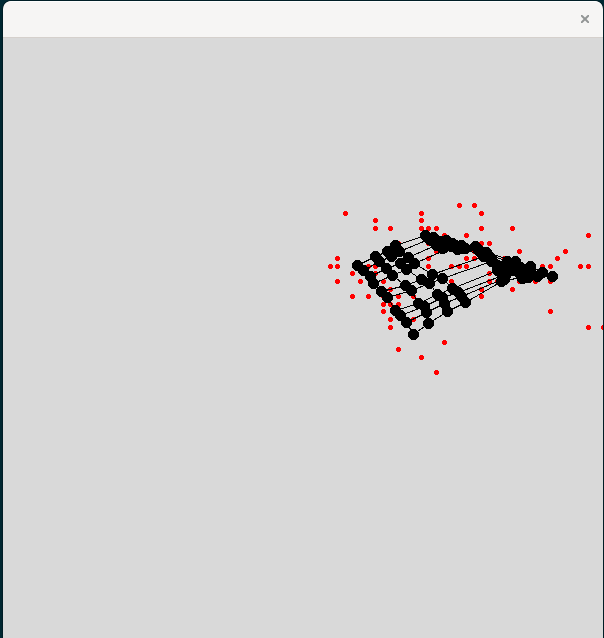
\includegraphics[width=.7\linewidth]{img/Screenshot from 2019-12-19 11-24-13.png}
\end{center}

\begin{center}
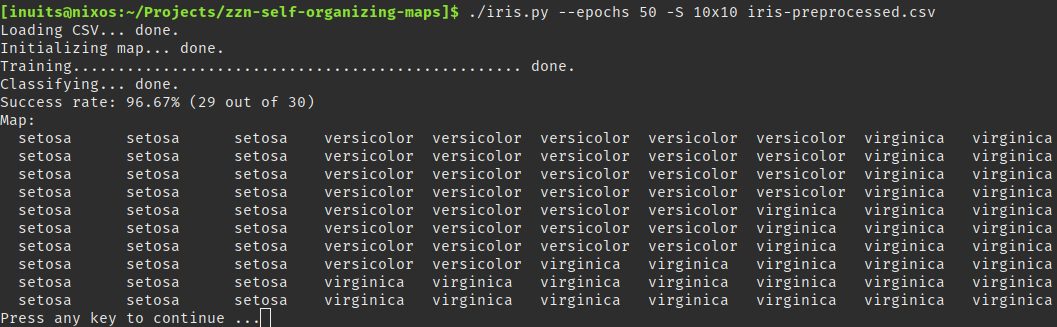
\includegraphics[width=1\linewidth]{img/Screenshot from 2019-12-19 11-25-49.png}
\end{center}

\newpage

\section{Závěr}
\label{sec:org3bc82d6}
Adaptovat tyto techniky pro jiné sady dat by mělo být triviální. Pro vizualizaci
vícerozměrných dat (např. MNIST) ale chybí implementace tzv. U-matrix
vizualizace, která zobrazuje ne absolutní umístění uzlu podle jednotlivých
souřadnic ale průměrnou vzdálenost uzlu od jeho sousedů, což je technika
použitelná pro libovolně vysoce dimenzionální data.

Naše implementace Kohonenovy mapy ale pracuje správně pro vizualizaci 2D dat a
pro klasifikaci libovolně rozměrných dat.

Zdrojový kód pro demonstrované programy je k dispozici na \url{https://github.com/zarybnicky/zzn-self-organizing-maps}.
\end{document}